\lecturechapter{Dienstag}{24. Mär}{24. März 2025}{Zermelo-Fraenkel-Axiome und Dedekindsche Schnitte}

\begin{nice-box}[Vorlesungsübersicht]
Diese Vorlesung bildet das Fundament für die rigorose Einführung der reellen Zahlen. Wir beginnen mit einer kurzen Clicker-Frage zum Vollständigkeitsaxiom, wiederholen das Fundierungsaxiom aus der Zermelo-Fraenkel-Mengenlehre und widmen uns dann der historischen und mathematischen Konstruktion von $\mathbb{R}$ mittels Dedekindscher Schnitte.
\end{nice-box}

\section{Einleitung und Clicker-Frage}

\begin{spoken-clean}[00:00:00 - 00:01:43]
Hallo und herzlich willkommen! Ich habe hier eine kleine Clicker-Einstiegsfrage, die Sie auf der Edu-App beantworten können. Das ist eine gute Gelegenheit, um sich kurz zu konzentrieren. Und wenn Sie das gemacht haben, sagen Sie doch noch kurz Ihrer Nachbarin oder Ihrem Nachbarn Hallo --- und dann bitte wählen.

Okay, gut. Wählen Sie noch schnell; 60 Antworten sollten wir schon noch hinkriegen. Okay, tipptopp! Sehr gut, fast 100\,\% richtig --- oder sogar 100\,\% richtig, ja, keine falschen Aussagen zumindest.
\end{spoken-clean}

\begin{meta-note}[Projizierter Inhalt: Clicker-Frage]
Auf dem Projektor wird die folgende Frage angezeigt:
\begin{center}
\textbf{Was sagt die folgende Aussage aus?}
\[
\forall X \Bigl( \bigl( X \subseteq \mathbb{R} \wedge X \neq \emptyset \wedge \exists r \in \mathbb{R} \; \forall x \in X \, (x \le r) \bigr) \implies \exists s \in \mathbb{R} \; \bigl( \forall x \in X \, (x \le s) \wedge \forall t \in \mathbb{R} \, ( \forall x \in X \, (x \le t) \implies s \le t ) \bigr) \Bigr)
\]
\end{center}
\begin{itemize}
    \item \textbf{Option 1:} Falls $X$ nichtleer und nach oben beschränkt ist, hat $X$ ein Infimum.
    \item \textbf{Option 2:} Falls $X$ nichtleer und nach oben beschränkt ist, hat $X$ ein Supremum. (Korrekte Antwort)
    \item \textbf{Option 3:} Falls $X$ nichtleer und nach unten beschränkt ist, hat $X$ ein Infimum.
    \item \textbf{Option 4:} Falls $X$ nichtleer und nach unten beschränkt ist, hat $X$ ein Supremum.
    \item \textbf{Option 5:} weiß nicht.
\end{itemize}
\end{meta-note}

\begin{math-stroke}[Das Vollständigkeitsaxiom in Prädikatenlogik]
Die auf dem Clicker gezeigte Formel formalisiert das Vollständigkeitsaxiom der reellen Zahlen:
\begin{equation}
\label{eq:vollstaendigkeit}
\forall X \subseteq \mathbb{R} \colon \Big( \bigl( X \neq \emptyset \land \exists r \in \mathbb{R} \; \forall x \in X \colon x \le r \bigr) \implies \exists s \in \mathbb{R} \colon \bigl( \forall x \in X \colon x \le s \land \forall t \in \mathbb{R} \, (\forall x \in X \colon x \le t \implies s \le t) \bigr) \Big)
\end{equation}

\begin{explanation-of-steps}[Strukturelle Aufschlüsselung der Formel]
Die Formel lässt sich logisch in zwei Hauptteile zerlegen:
\begin{enumerate}[label=\textbf{\arabic*.}]
    \item \textbf{Voraussetzung (Prämisse):} 
    \begin{itemize}
        \item $X \neq \emptyset$ bedeutet, dass die Teilmenge $X$ nicht leer ist.
        \item $\exists r \in \mathbb{R} \; \forall x \in X \colon x \le r$ bedeutet, dass $X$ nach oben beschränkt ist (mit einer oberen Schranke $r$).
    \end{itemize}
    \item \textbf{Konsequenz (Zielsatz):} Es existiert eine kleinste obere Schranke $s \in \mathbb{R}$ (das Supremum):
    \begin{itemize}
        \item $\forall x \in X \colon x \le s$ besagt, dass $s$ eine obere Schranke von $X$ ist.
        \item $\forall t \in \mathbb{R} \, (\forall x \in X \colon x \le t \implies s \le t)$ besagt, dass jede andere obere Schranke $t$ mindestens so groß ist wie $s$.
    \end{itemize}
\end{enumerate}
\end{explanation-of-steps}
\end{math-stroke}

\begin{spoken-clean}[00:01:43 - 00:03:45]
Genau, das ist es, was diese Aussage besagt. Man muss einfach mal genau schauen: Für alle Teilmengen $X$ von $\mathbb{R}$, so dass $X$ nicht leer ist --- also für alle $X$, so dass $X \subseteq \mathbb{R}$ und $X \neq \emptyset$ --- und es existiert ein $r$, so dass für alle $x \in X$ gilt $x \le r$, folgt, dass ein $s$ existiert, so dass für alle $x \in X$ gilt $x \le s$, und für alle $t$, so dass für alle $x \in X$ gilt $x \le t$, dann $s \le t$ ist. Das heißt, es existiert ein $s$, und dieses $s$ existiert als Supremum. Wenn ein $X$ also beschränkt ist, dann soll ein solches Supremum existieren --- das heißt eine obere Schranke, die die kleinste aller oberen Schranken ist. Okay.

Gut, dies nur als eine kleine Aufwärmübung. Wie Sie sehen, wird heute das Hauptthema der Vorlesung die Konstruktion der reellen Zahlen sein. Sie haben ja schon viel mit den reellen Zahlen gearbeitet und arbeiten wahrscheinlich auch aktuell viel damit, aber Sie haben noch nie eine volle Konstruktion davon gesehen. Das werden wir hier noch nachholen, wenn auch nicht in allen Details, weil das doch recht mühsam ist.

Genau. Aber zuerst möchte ich noch ganz kurz die Sache mit den Zermelo-Fraenkel-Axiomen anschauen. Moment mal...
\end{spoken-clean}

\section{Das Fundierungsaxiom (Regularitätsaxiom)}

\begin{spoken-clean}[00:03:45 - 00:05:48]
Die Zermelo-Fraenkel-Axiome --- einfach noch zur Erinnerung: Wir hatten die Axiome von Zermelo, das sind eigentlich die wichtigen, die einleuchtenden: das Axiom der Bestimmtheit, das Axiom der Elementarmengen, das Axiom der Aussonderung, das Axiom der Potenzmenge, das Axiom der Vereinigung, das Axiom der Auswahl und das Axiom des Unendlichen. Das ist so, wie es Zermelo formuliert hatte; wir haben das dann ausgeführt.

Letztes Mal haben wir dann noch die zwei zusätzlichen Axiome von Fraenkel hinzugefügt. Da hatten wir nicht mehr so viel Zeit. Das war das Ersetzungsaxiom und insbesondere auch noch das Fundierungsaxiom. Wir haben gesehen, dass diese ein bisschen technischerer Natur sind. Das Ersetzungsaxiom macht noch unmittelbar Sinn: Wir wollten, dass quasi Mengen, die durch Formeln bestimmt sind, auch tatsächlich Mengen sind --- so ungefähr.

Das Fundierungsaxiom war vielleicht ein bisschen schwieriger zugänglich. Ich kann das nochmals kurz wiederholen, da das letztes Mal ein bisschen zu kurz gekommen ist. Oh, was haben wir da noch? Das Fundierungsaxiom sagte uns aus: Für alle $x$, die nicht die leere Menge sind, existiert ein $y$, so dass $y \in x$ ist und außerdem der Durchschnitt von $y$ mit $x$ die leere Menge ist ($y \cap x = \emptyset$). Jetzt muss man da noch die Klammern richtig setzen. Genau.
\end{spoken-clean}

\begin{ai-global-state-checkpoint-invisible-content}
timestamp: 00:05:30, topic: Fundierungsaxiom und seine Konsequenzen, board_state: def:fundierungsaxiom
\end{ai-global-state-checkpoint-invisible-content}

\begin{math-stroke}[Das Fundierungsaxiom]
\begin{theorem}[Fundierungsaxiom / Regularitätsaxiom]\label{ax:fundierung}
Jede nicht-leere Menge $x$ enthält ein Element $y$, das disjunkt zu $x$ ist:
\begin{equation}
\label{eq:fundierungsaxiom}
\forall x \left( x \neq \emptyset \implies \exists y \left( y \in x \land y \cap x = \emptyset \right) \right)
\end{equation}
\end{theorem}

\begin{explanation-of-steps}[Konsequenzen des Fundierungsaxioms]
Das Fundierungsaxiom schließt zirkuläre Mengenstrukturen und unendliche Regresse aus:
\begin{enumerate}[label=\textbf{(\roman*)}]
    \item \textbf{Ausschluss von Selbstmitgliedschaft:} Keine Menge kann sich selbst als Element enthalten:
    \[
    x \notin x \quad \forall x
    \]
    \item \textbf{Ausschluss von Zyklen:} Es gibt keine zyklischen Elementbeziehungen der Form:
    \[
    x \in y \land y \in x
    \]
    \item \textbf{Ausschluss unendlicher Ketten:} Es existieren keine unendlichen absteigenden Ketten bezüglich der Elementrelation:
    \[
    x_0 \ni x_1 \ni x_2 \ni x_3 \ni \dots
    \]
\end{enumerate}
\end{explanation-of-steps}
\end{math-stroke}

\begin{didactic-insight}[Die Rolle des Fundierungsaxioms]
Das Fundierungsaxiom sorgt dafür, dass die "Mengenwelt" wohlfundiert ist. Es stellt sicher, dass jede Menge hierarchisch aus einfacheren Mengen aufgebaut ist, beginnend bei der leeren Menge $\emptyset$. Ohne dieses Axiom könnte man pathologische Objekte konstruieren, die sich selbst enthalten, was zwar nicht direkt zu Widersprüchen führt, aber die mathematische Struktur unnötig verkompliziert.
\end{didactic-insight}

\begin{spoken-clean}[00:05:48 - 00:08:20]
Also mit anderen Worten: Für jede Menge $x$, die nicht leer ist, existiert ein $y$, so dass kein Element von $y$ auch ein Element von $x$ ist. Gut, und insbesondere ein wichtiges Beispiel hiervon ist, wie wir gesehen haben: Es gibt keine unendlichen absteigenden Sequenzen von Mengen --- also $x_0$, das $x_1$ enthält, wobei diese Menge wiederum $x_2$ enthält, und diese $x_3$ und so weiter. Und es gibt keine Zyklen in Mengen, so dass etwa $x_0 \in x_1$, $x_1 \in x_2$ und so weiter bis $x_n \in x_0$. Insbesondere ist $x$ nicht in sich selbst enthalten, weil man sonst genau einen solchen Zyklus hätte.

Die Sache mit diesem Axiom ist: Das ist eigentlich wirklich von Mengentheoretikern für Mengentheoretiker gemacht. Die Mengen, die in der Alltagsmathematik oder der Mathematik, die wir normalerweise betreiben, vorkommen, erfüllen diese Eigenschaft ohnehin schon immer. Das heißt, es ist auch nicht so gemeint --- ich bin ja selbst kein Logiker ---, aber gemäß den Logikern funktioniert sehr vieles auch, wenn man dieses Axiom weglassen würde.

Aber konzeptuell macht es viele Sachen einfacher, insbesondere Beweise in der Mengenlehre, und es schließt pathologische Fälle aus, die sonst auftreten könnten. Es ist aber auch nicht "gefährlich": Das Axiom ist konsistent genau dann, wenn der Rest von Zermelo-Fraenkel konsistent ist. Das heißt, man riskiert nichts, wenn man es dazunimmt. Es gibt aber effektiv wohl auch Leute, die versuchen, ohne dieses Axiom zu arbeiten, um zu schauen, was man trotzdem alles beweisen kann.

Okay, das war es zu den Zermelo-Fraenkel-Axiomen. Nächste Woche kommt noch das Auswahlaxiom dran. Das ist noch ein wichtiges Axiom --- vielleicht das einzige Axiom von Zermelo-Fraenkel (oder eben ZF plus Auswahlaxiom), das ein ganz klein wenig streitbar ist oder von dem manche Leute sagen, sie wollen es nicht anwenden. Wenn man das Auswahlaxiom nicht verwenden möchte, kann es auch sehr hilfreich sein zu sehen, was man trotzdem beweisen kann. Aber ja: Ich wollte nur sagen, das Fundierungsaxiom gibt es auch noch, aber wichtig ist vor allem, dass man die anderen gut versteht --- die Existenz der leeren Menge, die Potenzmenge und so weiter.
\end{spoken-clean}

\begin{ai-global-state-checkpoint-invisible-content}
% timestamp: 00:11:00
% topic: Historischer Kontext der reellen Zahlen
% board_state: none
% next_goal: Axiome der reellen Zahlen
% open_loops: none
\end{ai-global-state-checkpoint-invisible-content}

\section{Historischer Kontext und Richard Dedekind}

\begin{spoken-clean}[00:08:20 - 00:10:45]
Soweit dazu. Heute kommen wir zum nächsten Thema. Wie gesagt: Nächste Woche kommt das Auswahlaxiom dran, deswegen sagt man oft "Zermelo-Fraenkel" für die Theorie ZF und "Zermelo-Fraenkel plus Axiom of Choice" (ZFC) für den Fall, dass man das Auswahlaxiom hinzunimmt. Das ist der Rahmen, in dem sich eigentlich ein Großteil der modernen Mathematik abspielt.

Jetzt aber zu den reellen Zahlen. Wir werden uns die Konstruktion von Richard Dedekind anschauen, also die Dedekindschen Schnitte. Das war, würde ich sagen, das erste moderne Fundament, eine formale Definition der reellen Zahlen. Richard Dedekind --- hier ein Foto --- stammte aus Braunschweig und war ein Student von Gauß. Was eben noch spannend ist: Er hat von 1858 bis 1862 hier an der ETH unterrichtet. Die ETH wurde ja 1854 gegründet, das heißt, ganz am Anfang der Geschichte der ETH war Richard Dedekind hier und hat Mathematik gelehrt. Es war auch in dieser Zeit, als er diese Dedekindschen Schnitte anscheinend entdeckt hat.

Es gibt einen Eintrag --- ich weiß nicht genau, ob in einem Brief oder einem Tagebuch, das finden Sie auch im Skript ---, wo er geschrieben hat, dass er wieder einmal an der ETH (oder dem Polytechnikum, wie es damals hieß) eine Vorlesung zur Analysis gegeben habe. Dabei sei ihm wieder klar geworden, wie wichtig es wäre, einmal saubere Grundlagen zu erarbeiten. Er hat daran gearbeitet und dann eben diese Dedekindschen Schnitte gefunden. Es macht also Sinn, dass wir Dedekind behandeln, weil das eben auch hier in der Nähe entdeckt worden ist. Ich glaube, das waren gute Zeiten damals: eine sehr spannende, neue technische Schule in der Schweiz und Richard Dedekind, der Vorlesungen gibt. Es wäre sicher spannend gewesen, hier dabei zu sein.
\end{spoken-clean}

\begin{meta-note}[Projizierter Inhalt: Richard Dedekind]
Auf der Folie wird ein Porträt von Richard Dedekind (1831–1916) gezeigt mit dem Titel \textbf{Konstruktion der reellen Zahlen} und dem Unterpunkt \textbf{Dedekindsche Schnitte}.
\end{meta-note}

\begin{spoken-clean}[00:10:45 - 00:13:30]
Gut, vielleicht noch ein bisschen zur Geschichte der reellen Zahlen. Die rationalen Zahlen sind ja etwas relativ Natürliches. Die ganzen Zahlen hatten wahrscheinlich schon die Steinzeitmenschen --- sie hatten zumindest eine Vorstellung von natürlichen Zahlen und Mengen. Rationale Zahlen kommen ins Spiel, sobald man anfängt zu dividieren und sich für Verhältnisse interessiert; das haben die Leute schon sehr früh gemacht. Ich glaube, bereits bei den Ägyptern und definitiv bei den Griechen wusste man dann, dass es auch irrationale Zahlen gibt. Ich glaube, bereits in Ägypten hatte man dieses Konzept, und Pythagoras und seine Schule hatten ja auch Beweise dafür.

Später wurde die Analysis entwickelt, eigentlich von Newton und Leibniz, aber auch später von Cauchy. Cauchy hat die Analysis dann schon sehr formal definiert, aber das wurde alles gemacht, ohne einen sauberen Begriff davon zu haben, was reelle Zahlen überhaupt sind. Das Ganze fiel dann so in das 19. Jahrhundert --- da waren auch Riemann und die anderen großen Namen ---, und sie alle merkten: Okay, wir brauchen eine gute, saubere Definition dessen, was eine reelle Zahl überhaupt ist.

Das fiel in die Zeit einer gewissen Grundlagenkrise in der Mathematik, die aber auch sehr fruchtbar war, so in der zweiten Hälfte des 19. Jahrhunderts. Zuerst hat man die reellen Zahlen definiert, aber dann gleichzeitig oder kurz danach hat man versucht, überhaupt erst einmal zu definieren, was eine ganze oder eine rationale Zahl ist. Das ist ja das, was wir bereits die vorherigen Male gemacht haben. Es gibt das Problem mit den ganzen Zahlen, dass man sie eigentlich gar nicht formal definieren kann --- zumindest nicht in dieser Prädikatenlogik erster Stufe. Deswegen haben wir eben dieses $\omega$, das eigentlich ganz gut ist und für uns ausreicht. Das war also die Zeit, in der man das versucht hat und in der die ganze Logik ihren Ursprung genommen hat. So viel zur Geschichte.
\end{spoken-clean}

\begin{ai-global-state-checkpoint-invisible-content}
% timestamp: 00:16:30
% topic: Axiome der reellen Zahlen
% board_state: def:reelle-zahlen-axiome
% next_goal: Das Vollständigkeitsaxiom und Dedekindsche Schnitte
% open_loops: none
\end{ai-global-state-checkpoint-invisible-content}

\section{Die Axiome der reellen Zahlen}

\begin{spoken-clean}[00:13:30 - 00:15:45]
Wir machen jetzt einen Sprung und definieren direkt die Axiome der reellen Zahlen. Wir haben hier wieder ein Axiomensystem. Unsere Signatur enthält $0, 1, +, \cdot$ und das Kleiner-als-Symbol ($<$). Das heißt auch hier wieder: $0$ und $1$ sind Konstanten, $+$ und $\cdot$ sind zwei binäre Funktionssymbole und $<$ ist ein binäres Relationssymbol.

Ein Punkt ist noch wichtig: Bei den Axiomen der reellen Zahlen bewegen wir uns bereits in der Zermelo-Fraenkel-Theorie. Um die reellen Zahlen überhaupt zu definieren, brauchen wir also bereits die Mengenlehre. Wir bewegen uns innerhalb der Mengenlehre und fügen jetzt einfach noch zusätzliche Axiome hinzu. Wir werden das gleich sehen.

Das erste Set von Axiomen kennen wir bereits: das sind die Körperaxiome. Ich werde die jetzt nicht an die Tafel schreiben, weil das sehr lang ist, aber Sie kennen sie ja: Die Addition muss assoziativ und kommutativ sein, $0$ ist neutral, und es existiert ein Inverses bezüglich der Addition. Für die Multiplikation gilt Analoges: Sie ist assoziativ und kommutativ, es existiert ein neutrales Element ($1$), und es gibt multiplikative Inverse für alle Elemente außer der Null. Schließlich haben wir die Verknüpfung von Multiplikation und Addition durch das Distributivgesetz, und wir fordern $0 \neq 1$. Das ist das erste Set von neun Axiomen, die unsere reellen Zahlen erfüllen sollen.

Dann kommt das nächste Set, das wir auch schon gesehen haben: das Set der dichten linearen Ordnung. Wir wollen also für alle $x$, dass $x$ nicht kleiner sein kann als es selbst (Irreflexivität), wir wollen Transitivität, und es soll eine lineare Ordnung sein. Zudem soll sie dicht sein und keine größten oder kleinsten Elemente haben. Okay, soweit haben wir das alles schon gesehen.
\end{spoken-clean}

\begin{meta-note}[Projizierter Inhalt: Axiome der reellen Zahlen]
Auf den Folien werden die Axiome der reellen Zahlen präsentiert:
\begin{center}
\textbf{Die Axiome der reellen Zahlen}
\end{center}
Die Signatur des Axiomensystems $\mathbb{R}$ der reellen Zahlen ist $\Sigma_{\mathbb{R}} = \{0, 1, +, \cdot, <\}$, wobei $0$ und $1$ Konstantensymbole sind, $+$ und $\cdot$ binäre Funktionssymbole sind und $<$ ein binäres Relationssymbol ist.
\begin{itemize}
    \item \textbf{Körperaxiome ($R_1$ bis $R_9$):} Assoziativität, Kommutativität, neutrale und inverse Elemente für $+$ und $\cdot$, Distributivgesetz, $0 \neq 1$.
    \item \textbf{Ordnungsaxiome ($R_{10}$ bis $R_{14}$):} Irreflexivität, Transitivität, lineare Ordnung, dichte Ordnung, keine Endpunkte.
\end{itemize}
\end{meta-note}

\begin{math-stroke}[Axiomensystem der reellen Zahlen]
Die Signatur der reellen Zahlen ist definiert als:
\[
\Sigma_{\mathbb{R}} := \{0, 1, +, \cdot, <\}
\]
Ein Modell der reellen Zahlen erfüllt die Axiome $R_1$ bis $R_{16}$ (angeordneter Körper mit dichter linearer Ordnung ohne Endpunkte).
\end{math-stroke}

\begin{spoken-clean}[00:15:45 - 00:17:40]
Jetzt kommen noch drei weitere Axiome dazu. Das erste haben wir so zwar noch nicht explizit hingeschrieben, aber wir kennen es eigentlich auch: Wir wollen jetzt einfach die Ordnung ($<$) mit $+$ und $\cdot$ verknüpfen --- wir wollen also, dass diese kompatibel sind. Das erste besagt: Wenn $x < y$ gilt, dann soll auch $x + z < y + z$ gelten. Wenn wir also Zahlen auf beiden Seiten addieren, soll das unsere Ordnung erhalten.

Das nächste Axiom sagt dasselbe für die Multiplikation. Da muss man ein bisschen sorgfältig sein, weil sich bei der Multiplikation mit einer negativen Zahl ja alles umkehrt. Also formulieren wir es so: Für alle $x$ und alle $y$ gilt: Wenn $x$ positiv ist ($x > 0$) und $y$ positiv ist ($y > 0$), dann soll auch $x \cdot y$ positiv sein.

Gut. Und bevor ich zum 17. Axiom komme --- das machen wir gleich an der Tafel ---: Das ist im Grunde das, was wir schon vorher gesehen haben. Ich möchte aber zuerst darauf hinweisen: Hier sieht man tatsächlich, dass wir Mengen brauchen, um diese Formel überhaupt zu formulieren. Wir brauchen "für alle Teilmengen $X$ von $\mathbb{R}$" und "für alle $x \in X$ existiert..." und so weiter. Das heißt, die Theorie der reellen Zahlen bzw. des Körpers der reellen Zahlen lebt in der Theorie von Zermelo-Fraenkel. Wir brauchen die Mengenlehre zwingend. Das ist anders als bei den vorherigen Axiomen; jene bilden eine Theorie für sich selbst, für die man eigentlich keine Mengenlehre benötigt --- das ist eine schwächere Formulierung. Aber für dieses 17. Axiom brauchen wir sie tatsächlich.
\end{spoken-clean}

\begin{meta-note}[Projizierter Inhalt: Kompatibilitätsaxiome]
Auf den Folien wird die Kompatibilität der Ordnung mit den algebraischen Operationen gezeigt:
\begin{itemize}
    \item \textbf{$R_{15}$:} $\forall x \forall y \forall z \, (x < y \implies x + z < y + z)$ (Kompatibilität von $<$ mit $+$)
    \item \textbf{$R_{16}$:} $\forall x \forall y \, (0 < x \wedge 0 < y \implies 0 < x \cdot y)$ (Kompatibilität von $<$ mit $\cdot$)
\end{itemize}
\end{meta-note}

\begin{math-stroke}[Das Vollständigkeitsaxiom]
Das Vollständigkeitsaxiom $R_{17}$ lautet:
\begin{equation}
\label{eq:vollstaendigkeit_axiom}
R_{17}\colon \quad \text{Jede nichtleere, nach oben beschränkte Teilmenge } X \subseteq \mathbb{R} \text{ hat ein Supremum.}
\end{equation}
\end{math-stroke}

\begin{spoken-clean}[00:17:40 - 00:20:15]
Was wir jetzt weiter machen: Der Körper $\mathbb{Q}$ der rationalen Zahlen erfüllt mit den üblichen Operationen und Relationen bereits die Axiome $R_1$ bis $R_{16}$. Aber $R_{17}$ gilt hier eben nicht; das haben Sie vielleicht schon einmal in der Analysis gesehen. Wir werden das später auch noch sehen.

Gut, und jetzt definieren wir einfach direkt, was ein Dedekindscher Schnitt ist. Ich weiß nicht, ob Sie das in der Analysis schon ein bisschen gesehen haben oder gar nicht? Okay, schauen wir es uns an. Die Idee ist folgende: Wir haben hier --- wenn wir uns das vorstellen --- die rationalen Zahlen $\mathbb{Q}$, und wie wir gesehen haben, gibt es da Lücken, zum Beispiel $\sqrt{2}$. Haben Sie alle schon gesehen, dass $\sqrt{2}$ nicht rational ist? Genau. Es gibt natürlich ganz viele von diesen Lücken, an denen einfach keine rationalen Zahlen sind.

Was man trotzdem machen kann: Man kann an diesen Stellen die Achse in zwei Teile teilen --- man hat dann einen linken Teil und einen rechten Teil. Und what wir jetzt tun: Wir definieren unsere reellen Zahlen direkt als die Möglichkeiten, unsere rationalen Zahlen in zwei Teile zu teilen. Das ist eigentlich die Idee der Dedekindschen Schnitte.
\end{spoken-clean}

\section{Dedekindsche Schnitte}

\begin{spoken-clean}[00:20:15 - 00:22:30]
Das Ziel von heute ist es also, solche reellen Zahlen, die $R_1$ bis $R_{17}$ erfüllen, zu konstruieren. Das machen wir eben über die Dedekindschen Schnitte --- "Dedekindsche Schnitte" ist wahrscheinlich korrekter, aber ich schreibe es etwas kürzer.

Wir konstruieren die reellen Zahlen ausgehend von den rationalen Zahlen. Wir gehen also davon aus, dass wir die rationalen Zahlen bereits haben. Ja?

\inlinemetanote{Dozent hört auf eine Frage aus dem Publikum}

Doch, aus der Topologie kann man natürlich auch eine Theorie machen. Aber wenn $R_1$ bis $R_{17}$ erfüllt sind, dann können Sie daraus nachher eine Topologie definieren, wenn Sie wollen --- das folgt dann daraus. Wenn Sie diese Axiome haben, folgt alles Weitere. Man kann natürlich noch mehr Strukturen auf $\mathbb{R}$ definieren, aber das sind dann Dinge, die aus diesen Axiomen folgen. Man kann die reellen Zahlen natürlich auch anders definieren, es gibt da verschiedene Möglichkeiten. Aber gut, machen wir jetzt die Dedekindschen Schnitte.
\end{spoken-clean}

\begin{math-stroke}[Definition des Dedekindschen Schnitts]
Der Körper der rationalen Zahlen $\mathbb{Q}$ erfüllt die Axiome $R_1$ bis $R_{16}$, jedoch nicht das Vollständigkeitsaxiom $R_{17}$.

\begin{definition}[Dedekindscher Schnitt]\label{def:dedekindscher-schnitt}
Ein \newterm{Dedekindscher Schnitt} ist eine Teilmenge $\alpha \subseteq \mathbb{Q}$, welche die folgenden drei Bedingungen erfüllt:
\begin{enumerate}[label=\textbf{(D\arabic*)}]
    \setcounter{enumi}{-1}
    \item \textbf{Nicht-Trivialität:} $\alpha \neq \emptyset$ und $\alpha \neq \mathbb{Q}$.
    \item \textbf{Abgeschlossenheit nach unten:} Falls $p \in \alpha$ und $q \in \mathbb{Q}$ mit $q < p$, dann ist auch $q \in \alpha$.
    \item \textbf{Offenheit nach oben (Kein Maximum):} Für jedes $p \in \alpha$ existiert ein $q \in \alpha$ mit $p < q$.
\end{enumerate}
\end{definition}
\end{math-stroke}

\begin{ai-global-state-checkpoint-invisible-content}
% timestamp: 00:22:00
% topic: Definition von Dedekindschen Schnitten
% board_state: def:dedekind-schnitt
% next_goal: Geometrische Intuition und Definition von R
% open_loops: none
\end{ai-global-state-checkpoint-invisible-content}

\begin{spoken-clean}[00:22:30 - 00:24:50]
Was wir bereits konstruiert haben, sind die ganzen Zahlen. Wir haben einfach gesagt: Das ist gleich $\omega$. Daraus kann man dann $\mathbb{Z}$ konstruieren. Das machen wir jetzt aber nicht im Detail. Im Prinzip nimmt man die natürlichen Zahlen und fügt die negativen Zahlen hinzu; man muss ein bisschen aufpassen, wie man das sauber formal macht, das finden Sie zum Beispiel im Buch. Und aus $\mathbb{Z}$ kann man dann $\mathbb{Q}$ konstruieren. Aber auch das machen wir jetzt nicht; das sind alles keine schwierigen Sachen, es ist einfach nur etwas länglich.

Wir gehen also von einem Modell der rationalen Zahlen aus. Präziser gesagt: Das besteht aus dem Bereich $\mathbb{Q}$, den Konstanten $0$ und $1$, den binären Funktionen $+$ und $\cdot$ und der binären Relation $<$. In diesem Modell wissen wir schon, dass die Axiome $R_1$ bis $R_{16}$ gelten. Aber $R_{17}$ gilt hier eben nicht --- das haben Sie vielleicht schon einmal in der Analysis gesehen. Wir werden das später auch noch sehen.

Gut, und jetzt definieren wir einfach direkt, was ein Dedekindscher Schnitt ist. Ein Dedekindscher Schnitt ist eine Teilmenge $\alpha \subseteq \mathbb{Q}$, so dass die folgenden Bedingungen erfüllt sind. Das heißt, unsere reellen Zahlen werden eigentlich eine Teilmenge der Potenzmenge von $\mathbb{Q}$ sein. Wir wollen, dass Folgendes erfüllt ist: \textbf{(D0)} --- $\alpha$ soll nicht die leere Menge sein und $\alpha$ soll nicht ganz $\mathbb{Q}$ sein.
\end{spoken-clean}

\begin{spoken-clean}[00:24:50 - 00:27:12]
Die zweite Bedingung ist \textbf{(D1)}: Falls $p \in \alpha$ liegt und $q$ eine rationale Zahl ist, so dass $q < p$ gilt, dann ist auch $q \in \alpha$. Das heißt, sobald eine Zahl $p$ in $\alpha$ ist, sind auch alle kleineren Zahlen in $\alpha$. Man sagt oft, die Menge ist "nach unten abgeschlossen".

Und das letzte Axiom, \textbf{(D2)}, besagt: Für jedes $p \in \alpha$ existiert ein $q \in \alpha$, so dass $p < q$ gilt. Mit anderen Worten: Wir wollen, dass $\alpha$ kein maximales Element enthält. Okay?

Genau. Und die Bemerkung dazu ist das, was ich vorher schon gesagt habe: Ein Dedekindscher Schnitt $\alpha$ teilt $\mathbb{Q}$ in zwei disjunkte Mengen. Wenn wir uns das hier anschauen --- hier haben wir $0$ und dort $1$, das ist unsere Zahlachse $\mathbb{Q}$ ---, dann sehen wir: Wenn wir hier $\alpha$ haben, dann ist alles, was kleiner ist, auch drin. Das heißt, nach links geht das so weit runter, wie man will. Aber hier muss es irgendwo aufhören, weil es ja nicht ganz $\mathbb{Q}$ ist. Es kann also nicht beliebig große Elemente enthalten. Wenn irgendein Element drin ist, ist links davon alles drin; wäre es also nach oben unbeschränkt, hätte man ganz $\mathbb{Q}$. Das heißt, die Schnitte müssen alle nach oben beschränkt sein.
\end{spoken-clean}

\begin{math-stroke}[Die Menge der reellen Zahlen \texorpdfstring{$\mathbb{R}$}{R}]
\begin{definition}[Reelle Zahlen]\label{def:reelle-zahlen-menge}
Wir definieren die Menge der reellen Zahlen $\mathbb{R}$ als die Menge aller Dedekindschen Schnitte über $\mathbb{Q}$:
\begin{equation}
\label{eq:reelle_zahlen_def}
\mathbb{R} := \{ \alpha \subseteq \mathbb{Q} \mid \alpha \text{ ist ein Dedekindscher Schnitt} \} \subseteq \mathcal{P}(\mathbb{Q})
\end{equation}
\end{definition}

\begin{center}
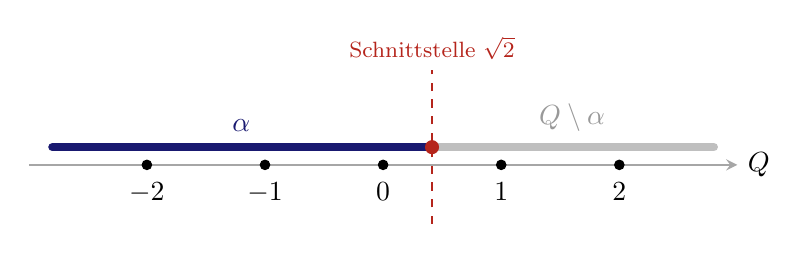
\begin{tikzpicture}[scale=1.5]
    % Q-Axis
    \draw[thick, ->, >=stealth, draw=gray!70] (-3, 0) -- (3, 0) node[right] {$\mathbb{Q}$};
    
    % Cut point (dashed line)
    \draw[dashed, thick, draw=BrickRed] (0.414, -0.5) -- (0.414, 0.8) node[above, text=BrickRed] {\footnotesize Schnittstelle $\sqrt{2}$};
    
    % The set \alpha (left side, shaded/thick)
    \draw[line width=3pt, MidnightBlue, line cap=round] (-2.8, 0.15) -- (0.364, 0.15);
    \node[MidnightBlue, above] at (-1.2, 0.2) {$\alpha$};
    
    % The complement \mathbb{Q} \setminus \alpha (right side)
    \draw[line width=3pt, gray!50, line cap=round] (0.464, 0.15) -- (2.8, 0.15);
    \node[gray!80, above] at (1.6, 0.2) {$\mathbb{Q} \setminus \alpha$};
    
    % Empty circle at the gap
    \draw[fill=white, thick, BrickRed] (0.414, 0.15) circle (0.05cm);
    
    % Labels for rational points
    \filldraw[black] (-2,0) circle (0.04cm) node[below=0.1cm] {$-2$};
    \filldraw[black] (-1,0) circle (0.04cm) node[below=0.1cm] {$-1$};
    \filldraw[black] (0,0) circle (0.04cm) node[below=0.1cm] {$0$};
    \filldraw[black] (1,0) circle (0.04cm) node[below=0.1cm] {$1$};
    \filldraw[black] (2,0) circle (0.04cm) node[below=0.1cm] {$2$};
\end{tikzpicture}
\end{center}
\end{math-stroke}

\begin{spoken-clean}[00:27:12 - 00:29:18]
Man sieht es also so: Nach oben ist der Schnitt offen --- es gibt kein größtes Element. Wir haben hier $\alpha$ und dort $\mathbb{Q} \setminus \alpha$. Wir schneiden also wirklich die Zahlgerade der rationalen Zahlen in zwei Stücke. Deswegen der Name "Dedekindscher Schnitt".

Wir definieren jetzt einfach als Menge $\mathbb{R}$ die Menge aller Dedekindschen Schnitte von $\mathbb{Q}$. Als Nächstes hätten wir gerne, dass die rationalen Zahlen in $\mathbb{R}$ enthalten sind. Hat jemand eine Idee, wie man das bewerkstelligen könnte? Oder wie sieht man natürlicherweise $\mathbb{Q}$ als Teilmenge von $\mathbb{R}$? Wie kann man eine rationale Zahl als Dedekindschen Schnitt interpretieren? Ja?

\inlinemetanote{ein Student antwortet: \qt{Die Menge der Zahlen, die kleiner sind als die Zahl}}

Genau! Wir können die Menge aller rationalen Zahlen anschauen, die strikt kleiner als eine gegebene Zahl sind. Für ein $p \in \mathbb{Q}$ definieren wir also $\alpha_p$ als die Menge aller $q \in \mathbb{Q}$, so dass $q < p$.
\end{spoken-clean}

\begin{spoken-clean}[00:29:18 - 00:30:51]
Wir müssen jetzt noch beweisen, dass das tatsächlich ein Dedekindscher Schnitt ist. Machen wir das mal gründlich. Also: \textbf{(D0)} ist erfüllt, die Menge ist nicht leer --- man kann immer kleinere Zahlen finden. Dann müssen wir \textbf{(D1)} zeigen, aber das ist auch klar: Wenn $q \in \alpha_p$ ist und $r \in \mathbb{Q}$ mit $r < q$, dann folgt aus $r < q$ und $q < p$ sofort $r < p$, und somit ist auch $r \in \alpha_p$. Da steckt also nicht viel dahinter.

Und dann noch das Letzte: Wir müssen zeigen, dass es kein größtes Element hat. Aber auch das ist nicht schwierig. Wenn wir ein $q \in \alpha_p$ haben, dann nehmen wir als $r$ einfach die Mitte zwischen $p$ und $q$, also $r = \frac{p+q}{2}$. Das ist wieder eine rationale Zahl. Dann liegt $r$ zwischen $q$ und $p$, das heißt $q < r$ und $r \in \alpha_p$.

Damit erhalten wir eine Injektion von $\mathbb{Q}$ in die reellen Zahlen. Aber die Sache ist die: Nicht alle Dedekindschen Schnitte sind von dieser Form --- die meisten, wie wir schlussendlich sehen werden, sind es nicht. Nehmen wir zum Beispiel $\sqrt{2}$ gewissermaßen. Wie könnte man $\sqrt{2}$ als Dedekindschen Schnitt definieren? Hat jemand eine Idee? Ja?

\inlinemetanote{ein Student antwortet: \qt{Die Menge aller rationalen Zahlen, deren Quadrat kleiner als zwei ist}}

Genau.
\end{spoken-clean}

\begin{spoken-clean}[00:30:51 - 00:32:12]
Schauen wir es uns an. Wir können zuerst sagen: Elemente in $\mathbb{R} \setminus \mathbb{Q}$ heißen irrational. Als Beispiel können wir den Dedekindschen Schnitt $\alpha$ anschauen, der aus allen $p \in \mathbb{Q}$ besteht, für die gilt: $p < 0$ oder $p^2 < 2$. Das definieren wir als $\sqrt{2}$.

Jetzt müsste man natürlich noch beweisen, dass das tatsächlich ein Dedekindscher Schnitt ist. Und später müssten wir eine Multiplikation definieren und zeigen, dass das Produkt dieser Zahl mit sich selbst tatsächlich $2$ ergibt. Das ist diese Woche auf dem Übungsblatt. Es ist nicht schwierig, aber es ist gut, so etwas einmal selbst zu machen.

Um zu zeigen, dass das kein rationaler Schnitt ist, kann man zeigen, dass es eben keine rationale Zahl gibt, deren Quadrat $2$ ist. Das wollen wir doch noch einmal beweisen. Die Behauptung ist: Es gibt keine Zahl $\frac{p}{q} \in \mathbb{Q}$ (mit $p, q \in \mathbb{Z}$), so dass $(\frac{p}{q})^2 = 2$ ist.
\end{spoken-clean}

\begin{spoken-clean}[00:32:12 - 00:34:33]
Der Beweis, den man normalerweise sieht, verwendet die Primfaktorzerlegung; den haben Sie vielleicht schon einmal gesehen. Wir schauen uns hier einen Beweis an, der von Dedekind selbst stammt --- deswegen ist er für diesen Hörsaal und dieses Thema vielleicht besonders passend.

Wir führen einen Widerspruchsbeweis. Nehmen wir an, es existieren solche $p, q \in \mathbb{Z}$. Wir können annehmen, dass es natürliche Zahlen sind, da das Quadrat ohnehin positiv ist; wir können also gut annehmen, dass $p, q \in \mathbb{N}$ liegen, so dass $\frac{p^2}{q^2} = 2$ ist. Das heißt mit anderen Worten: $p^2 - 2q^2 = 0$.

Wir nehmen nun an, dass $q \in \mathbb{N}$ die kleinste natürliche Zahl ist, die das erfüllt. Das heißt, $q$ ist die kleinste Zahl, so dass $2q^2$ eine Quadratzahl ist. Was wir hier sehen: Es muss $q < p$ gelten. (Nein, andersrum: $q < p$, weil wenn wir $q^2$ mit $2$ multiplizieren, bekommen wir $p^2$. Das passt.) Und wir wissen aber auch, dass $p < 2q$ ist (da $p^2 = 2q^2 < 4q^2$).
\end{spoken-clean}

\begin{spoken-clean}[00:34:33 - 00:35:55]
Jetzt definieren wir $q' := p - q$ und $p' := 2q - p$. Das sind beides positive Zahlen. Wegen unserer Annahme haben wir hier, dass $q'$ wieder positiv ist, und es gilt $0 < q' < q$.

Was wir jetzt tun: Wir zeigen einfach, dass $2(q')^2$ auch wieder ein Quadrat ist. Dazu rechnen wir $(p')^2 - 2(q')^2$ aus. Wir setzen die Definitionen ein:
\[ (p')^2 = (2q - p)^2 = 4q^2 - 4pq + p^2 \]
Und für den zweiten Teil:
\[ -2(q')^2 = -2(p - q)^2 = -2(p^2 - 2pq + q^2) = -2p^2 + 4pq - 2q^2 \]
Wenn wir das zusammenzählen, erhalten wir:
\[ (4q^2 - 2q^2) + (p^2 - 2p^2) = 2q^2 - p^2 \]
Da wir aber wissen, dass $p^2 - 2q^2 = 0$ ist, ist auch dieser Ausdruck $0$. Das heißt, $2(q')^2 = (p')^2$ ist tatsächlich wieder eine Quadratzahl.
\end{spoken-clean}

\begin{spoken-clean}[00:35:55 - 00:37:08]
Das ist aber ein Widerspruch zur Minimalität von $q$, da wir eine kleinere Zahl $q'$ gefunden haben, die dieselbe Eigenschaft erfüllt. Und das beendet den Beweis.

Es ist immer gut, hie und da einen Rechenfehler einzubauen --- oder zumindest so zu tun ---, dann beginnen die Leute wieder mitzudenken. Sehr gut! Aber genau, jetzt machen wir eine Pause und fahren um Viertel nach wieder fort.

Hier noch eine kleine Ergänzung zu dem, was wir vor der Pause kurz gemacht haben: Wir wissen, dass $p < 2q$ ist; das folgt direkt daraus, dass $p^2 = 2q^2$ ist. Zusammen mit $q < p$ folgt dann, dass $q' = p - q$ tatsächlich zwischen $0$ und $q$ liegt. Man braucht also diese beiden Ungleichungen.
\end{spoken-clean}

\section{Körperoperationen auf den reellen Zahlen}

\begin{spoken-clean}[00:37:08 - 00:39:28]
Gut. Als Nächstes wollen wir die Körperoperationen auf unseren Dedekindschen Schnitten definieren. Das Ziel ist es nun, eine Körperstruktur auf $\mathbb{R}$ zu definieren. Idealerweise wollen wir natürlich, dass diese die Körperstruktur von $\mathbb{Q}$ --- das wir jetzt als Teilmenge von $\mathbb{R}$ aufgefasst haben --- erweitert. Die Einschränkung auf $\mathbb{Q}$ soll also die übliche Körperstruktur ergeben.

Beginnen wir mit der Addition. Das soll eine binäre Funktion auf $\mathbb{R}$ sein. Wie müssen wir $\alpha + \beta$ definieren? Hat jemand eine Idee, wie man das sinnvoll machen könnte? Ja?

\inlinemetanote{ein Student antwortet: \qt{Man addiert einfach alle Elemente}}

Ja, genau! Wir nehmen einfach alle Summen $p + q$, wobei $p \in \alpha$ und $q \in \beta$. Wir nehmen also alle möglichen Kombinationen; das ergibt eine neue Menge, und die definieren wir als die Summe.

Das Erste, was wir prüfen müssen, ist, ob das wieder ein Dedekindscher Schnitt ist. Schnell überlegen: Ist das wieder ein Schnitt? Machen wir es mal. Ich kann es kurz erklären, aber solche Sachen macht man in der Regel am besten einmal alleine. Das Lemma lautet: $\alpha + \beta$ ist ein Dedekindscher Schnitt.
\end{spoken-clean}

\begin{spoken-clean}[00:39:28 - 00:40:51]
Der Beweis: Wir müssen alle Axiome nachprüfen. \textbf{(D0)} ist eigentlich klar: Wir wissen, dass $\alpha$ und $\beta$ beide nicht leer sind. Es gibt also ein $p \in \alpha$ und ein $q \in \beta$. Daraus folgt, dass $p + q \in \alpha + \beta$ liegt, die Summe ist also nicht leer.

Dann müssen wir zeigen, dass sie nicht ganz $\mathbb{Q}$ entspricht. Dazu nehmen wir ein Element $r \in \mathbb{Q}$, das nicht in $\alpha$ liegt, und ein $s \in \mathbb{Q}$, das nicht in $\beta$ liegt. Dann gilt für alle $p \in \alpha$ und alle $q \in \beta$, dass $p < r$ und $q < s$ ist. Das muss für alle $p$ und $q$ gelten, weil sonst $r$ in $\alpha$ oder $s$ in $\beta$ enthalten wäre. Somit folgt, dass $p + q < r + s$ ist. Das heißt, $r + s$ kann nicht in $\alpha + \beta$ liegen, womit die Summe nicht ganz $\mathbb{Q}$ ist.

Dann müssen wir sehen, dass sie nach unten abgeschlossen ist (\textbf{D1}). Dazu nehmen wir ein $r = p + q \in \alpha + \beta$ und ein $s \in \mathbb{Q}$ mit $s < r$. Wir nehmen an, $p \in \alpha$ und $q \in \beta$. Wir können dann ein $t$ so wählen, dass $s = t + q$ ist. Dann folgt aber, dass $t < p$ ist, und somit ist $t$ insbesondere in $\alpha$. Daraus folgt, dass $s = t + q$ auch wieder in $\alpha + \beta$ liegt.
\end{spoken-clean}

\begin{spoken-clean}[00:40:51 - 00:43:03]
Und dann müssen wir noch zeigen, dass es kein maximales Element gibt (\textbf{D2}). Wie können wir das machen? Hat jemand einen Vorschlag? Ja?

\inlinemetanote{ein Student antwortet: \qt{Es gab ja davor schon keins}}

Genau! Es gab schon vorher keines, dann gibt es auch in der Summe keines. Wenn wir ein $r = p + q \in \alpha + \beta$ haben (mit $p \in \alpha, q \in \beta$), dann gibt es ein $p' \in \alpha$ mit $p < p'$. Daraus folgt, dass $r = p + q < p' + q =: r'$ ist, und $r'$ ist immer noch in $\alpha + \beta$. Es gibt hier also kein maximales Element.

Okay. Das Nullelement haben wir ja bereits: Das sind alle $p \in \mathbb{Q}$, so dass $p < 0$ ist. Jetzt ist die Frage: Wie können wir das Negative von $\alpha$ nehmen? Was ist $-\alpha$? Für $\alpha \in \mathbb{R}$ definieren wir $-\alpha$ als den Dedekindschen Schnitt gegeben durch... wie könnte man das machen? Ja?

\inlinemetanote{ein Student antwortet: \qt{Spiegelung an der Null}}

Ja, genau. Man hätte gerne so etwas wie alles auf der anderen Seite, aber negativ genommen. Damit sich das dann immer zu etwas Kleinerem addiert... aber das ist ein bisschen schwierig, weil wir ja auch hier wieder die Offenheit nach oben brauchen. Aber genau das ist die Idee.
\end{spoken-clean}

\begin{spoken-clean}[00:43:03 - 00:44:52]
Ja?

\inlinemetanote{ein Student antwortet: \qt{Alle p, so dass p + q < 0 für alle q in alpha}}

Ah ja, das könnte man auch machen. Wir können sagen: Wir nehmen alle $p \in \mathbb{Q}$, so dass für alle $q \in \alpha$ gilt: $q + p < 0$. Das ist im Prinzip genau die Idee mit dem Spiegeln, man kann es nur anders hinschreiben. Man muss dann wieder prüfen, dass das tatsächlich ein Dedekindscher Schnitt ist.

Somit können wir auch subtrahieren. Und dann können wir sagen, was es heißt, größer oder kleiner als $0$ zu sein. Wir sagen: $\alpha > 0$, falls... was wäre ein einfaches Kriterium? Ja?

\inlinemetanote{ein Student antwortet: \qt{Wenn die Null im Schnitt enthalten ist}}

Wir sollten aufpassen, dass $-0$ dann auch noch ein Dedekindscher Schnitt ist... ich war da gerade zu schnell. Kurz überlegen: Hat jemand eine bessere Definition direkt? Ja?

\inlinemetanote{ein Student antwortet: \qt{Q ohne alpha, wo wir die Kehrwerte nehmen}}

Ja, aber das ist kein allgemeiner... dann haben wir die falsche Seite. Wenn wir davon das Komplement nehmen, ist es kein Dedekindscher Schnitt mehr, weil das ja bis zu einer bestimmten Zahl geht.
\end{spoken-clean}

\begin{spoken-clean}[00:44:52 - 00:46:05]
Ich schaue mal schnell nach... ich glaube, das Problem tritt nur bei der Null auf. Okay, ich überlege mir das sonst noch einmal schnell, oder Sie überlegen es sich, und ich schreibe es nachher per Mail --- das ist einfacher. Ich habe das gerade zu schnell überlegt, und solche Sachen an der Wandtafel zu machen, ist nicht immer ganz einfach. Vielleicht kommt es mir später wieder in den Sinn.

Machen wir es so: Wir sagen $\alpha > 0$, falls $0 \in \alpha$ enthalten ist. Und $\alpha < 0$, falls $-\alpha > 0$ ist. "Größer-gleich" ist dann natürlich klar.

Und jetzt zur Multiplikation. Da können wir sagen: Wir multiplizieren mit $-1$, das geht vielleicht ganz gut. Was für Ideen gibt es sonst für die Multiplikation? Ja?

\inlinemetanote{ein Student antwortet: \qt{Wie bei der Addition}}

Genau, das ist die Grundidee. Das Problem sind halt wieder die negativen Zahlen. Wenn beide positiv sind, ist das der richtige Weg. Da braucht es eine mühsame Fallunterscheidung: Falls $\alpha, \beta \ge 0$ sind, definieren wir $\alpha \cdot \beta$ als die Menge aller $p \cdot q$, wobei $p \in \alpha, q \in \beta$ und $p, q \ge 0$ sind, vereinigt mit allen negativen rationalen Zahlen. Das ist der erste Fall.
\end{spoken-clean}

\begin{spoken-clean}[00:46:05 - 00:49:12]
Wenn beide negativ sind, ist es ähnlich: Dann nehmen wir einfach das Produkt der Negativen, dann geht es auch wieder auf. Also: Falls $\alpha, \beta \le 0$ sind, definieren wir $\alpha \cdot \beta$ als $(-\alpha) \cdot (-\beta)$. Und entsprechend: Falls $\alpha \ge 0$ und $\beta \le 0$ ist, sagen wir $\alpha \cdot \beta = -(\alpha \cdot (-\beta))$. Und falls schließlich $\alpha \le 0$ und $\beta \ge 0$ ist, definieren wir $\alpha \cdot \beta = -((-\alpha) \cdot \beta)$.

Das ist das Mühsame mit den negativen Zahlen. Deswegen ist die Sache im Skript nur für die positiven reellen Zahlen aufgeschrieben und der Rest wird den Lesenden überlassen --- aber das lässt die Sache ein bisschen zu schön erscheinen.

Gut. Jetzt müsste man überprüfen, dass die Körperaxiome alle erfüllt sind. Man müsste also prüfen, dass das alles Dedekindsche Schnitte sind und dass alle Axiome gelten. Sie können sich vorstellen, dass das eine sehr lange Angelegenheit ist. Wir werden das jetzt nicht die nächsten drei Lektionen hier an der Tafel machen. Ich erwarte auch nicht von Ihnen, dass Sie das tun, aber falls Sie einmal eine lange Zugfahrt haben: Das wäre eine gute Übung. Zeigen Sie, dass die Dedekindschen Schnitte mit diesen Operationen die Körperaxiome erfüllen.
\end{spoken-clean}

\begin{spoken-clean}[00:49:12 - 00:52:12]
Das wäre der erste Schritt. Als Nächstes brauchen wir noch eine Ordnung auf den Dedekindschen Schnitten. Die Ordnung ist relativ natürlich definiert: Wenn wir $\alpha, \beta \in \mathbb{R}$ haben, wie definieren wir $\alpha < \beta$? Haben Sie eine Idee? Ja?

\inlinemetanote{ein Student antwortet: \qt{alpha ist eine echte Teilmenge von beta}}

Genau! $\alpha \subsetneq \beta$. Das wäre etwas weniger lang zu beweisen, aber man müsste es auch machen --- vielleicht für die Rückfahrt: Zeigen Sie, dass dadurch auch die Ordnungsaxiome erfüllt sind. Aber diese Art von Beweisen ist oft so: Man überprüft einfach alles, es stecken keine wirklich "interessanten" Argumente drin, es dauert nur sehr lange.

Was wir aber noch im Detail beweisen wollen, ist das Axiom $R_{17}$, also die Vollständigkeit. Der Satz lautet: Die reellen Zahlen $\mathbb{R}$ erfüllen $R_{17}$, das heißt, jede nichtleere, nach oben beschränkte Teilmenge $X \subseteq \mathbb{R}$ hat ein Supremum.

Der Beweis dafür ist wirklich natürlich. Wir konstruieren das Supremum $\beta$ einfach als die Vereinigung aller Dedekindschen Schnitte in $X$:
\[ \beta := \bigcup X = \{ p \in \mathbb{Q} \mid \exists \alpha \in X \text{ mit } p \in \alpha \} \]
Wir müssen beweisen, dass das ein Dedekindscher Schnitt ist und dass es tatsächlich das Supremum ist.
\end{spoken-clean}

\begin{spoken-clean}[00:52:12 - 00:55:29]
Zuerst einmal: $\beta$ ist ein Dedekindscher Schnitt. Da zeigen wir wieder alle drei Bedingungen. \textbf{(D0)}: Es ist klar, dass $\beta$ nicht leer ist, da $X$ nicht leer ist und somit mindestens einen nichtleeren Schnitt enthält. Um zu zeigen, dass es nicht ganz $\mathbb{Q}$ ist, verwenden wir, dass $X$ nach oben beschränkt ist. Es gibt also eine obere Schranke $\gamma \in \mathbb{R}$, so dass für alle $\alpha \in X$ gilt $\alpha \subseteq \gamma$. Da $\gamma \neq \mathbb{Q}$, gibt es ein $q \in \mathbb{Q} \setminus \gamma$, und dieses $q$ kann dann auch nicht in der Vereinigung $\beta$ liegen.

\textbf{(D1)}: Sei $p \in \beta$ und $q \in \mathbb{Q}$ mit $q < p$. Wir müssen zeigen, dass $q \in \beta$ ist. Da $p \in \beta$, existiert ein $\alpha \in X$, das $p$ enthält. Da $\alpha$ ein Dedekindscher Schnitt ist, folgt aus $q < p$ sofort $q \in \alpha$, und somit ist $q$ auch in der Vereinigung $\beta$.

\textbf{(D2)}: Sei $p \in \beta$. Wir wollen ein größeres Element in $\beta$ finden. Es existiert ein $\alpha \in X$ mit $p \in \alpha$. Da $\alpha$ ein Dedekindscher Schnitt ist, existiert ein $q \in \alpha$ mit $p < q$. Dann ist $q$ aber auch in der Vereinigung $\beta$ enthalten. Das heißt, $\beta$ ist tatsächlich ein Dedekindscher Schnitt.
\end{spoken-clean}

\begin{spoken-clean}[00:55:29 - 00:58:07]
Jetzt müssen wir noch zeigen, dass es die kleinste obere Schranke ist. Dass es eine obere Schranke ist, ist klar: Jedes $\alpha \in X$ ist nach Definition eine Teilmenge der Vereinigung, also $\alpha \le \beta$.

Um zu zeigen, dass es die kleinste ist, nehmen wir an, es gäbe ein $\gamma \in \mathbb{R}$ mit $\gamma < \beta$. Wir wollen zeigen, dass $\gamma$ dann keine obere Schranke mehr sein kann. Wenn $\gamma < \beta$ ist, dann ist $\gamma$ eine echte Teilmenge von $\beta$. Es gibt also ein $p$, das in $\beta$ liegt, aber nicht in $\gamma$. Da $p \in \beta$, existiert ein $\alpha \in X$ mit $p \in \alpha$. Da $\alpha$ ein Element enthält, das nicht in $\gamma$ ist, kann $\alpha$ keine Teilmenge von $\gamma$ sein. Somit ist $\gamma < \alpha$, was bedeutet, dass $\gamma$ keine obere Schranke für $X$ ist. Das beendet den Beweis.

Ich möchte zum Abschluss noch zwei Sachen erwähnen. Es gibt noch andere bekannte Konstruktionen der reellen Zahlen. Die wohl bekannteste ist die über Cauchy-Folgen. Das Problem mit den rationalen Zahlen ist ja, dass Cauchy-Folgen dort nicht unbedingt konvergieren. Man kann nun künstlich erzwingen, dass alle Cauchy-Folgen konvergieren, indem man Äquivalenzklassen von Cauchy-Folgen betrachtet. Das ist die zweite klassische Konstruktion; sie wurde fast zeitgleich mit der von Dedekind publiziert.
\end{spoken-clean}

\begin{spoken-clean}[00:58:07 - 01:02:09]
Es gibt auch eine Konstruktion, die weniger bekannt und weniger klassisch ist --- sie stammt erst aus jüngerer Zeit. Wir haben sie diese Woche auf dem Übungsblatt, und es ist eine sehr nette Konstruktion: Man konstruiert die reellen Zahlen dabei direkt aus den ganzen Zahlen. Man muss gar nicht erst den Umweg über die rationalen Zahlen gehen.

Die Idee ist, Äquivalenzklassen von sogenannten quasilinearen Funktionen zu betrachten. Das sind Funktionen $f \colon \mathbb{Z} \to \mathbb{Z}$, für die gilt, dass die Menge der Werte $f(n+m) - f(n) - f(m)$ (für alle $n, m \in \mathbb{Z}$) endlich ist. Wäre $f$ linear, wäre dieser Ausdruck immer $0$. Wir schauen uns aber quasilineare Funktionen an, bei denen diese Abweichung von der Linearität beschränkt bleibt.

Man kann zeigen, dass geeignete Äquivalenzklassen solcher Funktionen ebenfalls die reellen Zahlen ergeben. Das ist besonders elegant, weil man direkt bei den ganzen Zahlen anfangen kann. Ich empfehle Ihnen, sich diese Übung einmal anzuschauen, weil das sehr interessant und kein Standardstoff ist.

Gut, vielen herzlichen Dank fürs Kommen und eine gute Woche!
\end{spoken-clean}

\begin{math-stroke}[Alternative Konstruktionen der reellen Zahlen]
Neben der Konstruktion von Richard Dedekind über Dedekindsche Schnitte existieren weitere mathematische Verfahren zur Konstruktion von $\mathbb{R}$ aus $\mathbb{Q}$ bzw. $\mathbb{Z}$:

\begin{itemize}
    \item \textbf{Konstruktion über Cauchy-Folgen (Cantor):}
    Die reellen Zahlen werden als Äquivalenzklassen von Cauchy-Folgen rationaler Zahlen definiert. Zwei Cauchy-Folgen $(a_n)_{n \in \mathbb{N}}$ und $(b_n)_{n \in \mathbb{N}}$ heißen äquivalent, falls ihre Differenz eine Nullfolge ist:
    \[
    (a_n) \sim (b_n) \iff \lim_{n \to \infty} (a_n - b_n) = 0.
    \]
    Diese Konstruktion vervollständigt den metrischen Raum $(\mathbb{Q}, d_{\text{Eucl}})$.

    \item \textbf{Konstruktion über quasilineare Funktionen (Eudoxus-Reelle-Zahlen):}
    Diese moderne, elegante Konstruktion definiert die reellen Zahlen direkt aus den ganzen Zahlen $\mathbb{Z}$ ohne den Umweg über die rationalen Zahlen $\mathbb{Q}$. Wir betrachten Äquivalenzklassen von \newterm{quasilinearen Funktionen} $f \colon \mathbb{Z} \to \mathbb{Z}$, für die gilt, dass die Menge:
    \[
    \{ f(n+m) - f(n) - f(m) \mid n, m \in \mathbb{Z} \}
    \]
    endlich ist.
\end{itemize}
\end{math-stroke}

% [SYSTEM] Refinement complete